\tikzset{    
    node1/.style={
        above right
    }
}
\scalebox{0.5}{
    \begin{tikzpicture}
        \node[node1,label={$A \cup B$}]           at (0,0)  {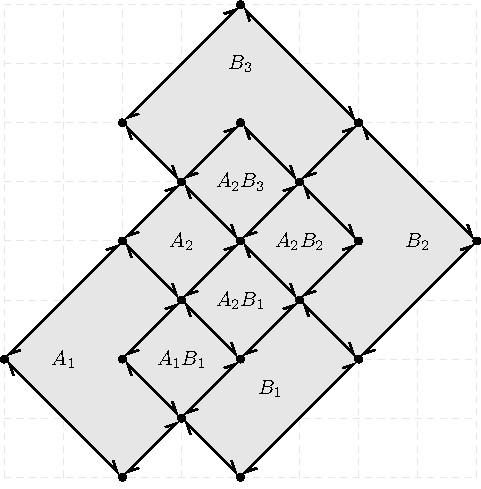
\includegraphics[scale=0.75]{figures/04/DCELUnion}};
        \node[node1,label={$A \cap B$}]           at (7,0)  {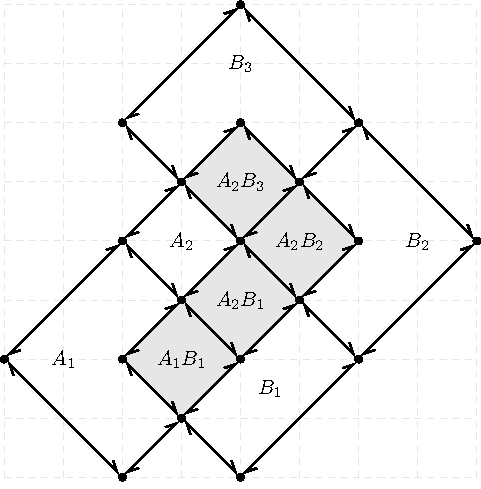
\includegraphics[scale=0.75]{figures/04/DCELIntersection}};
        \node[node1,label={$A \setminus B$}]      at (14,0) {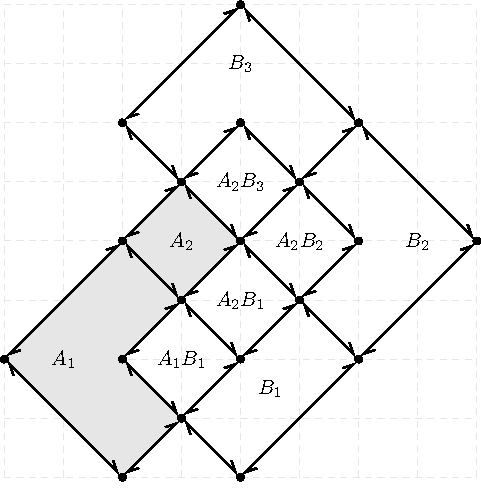
\includegraphics[scale=0.75]{figures/04/DCELDiffA}};
        \node[node1,label={$B \setminus A$}]      at (21,0) {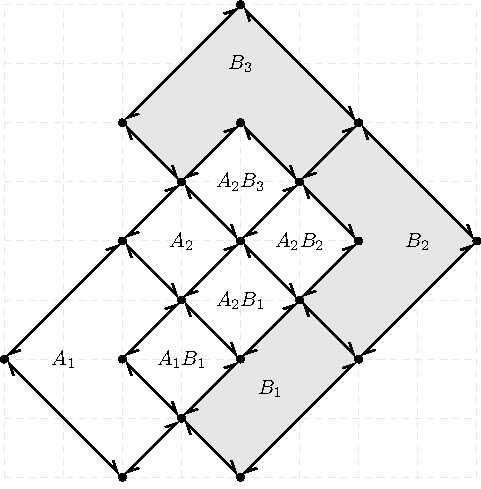
\includegraphics[scale=0.75]{figures/04/DCELDiffB}};
        \node[node1,label={$A \bigtriangleup B$}] at (28,0) {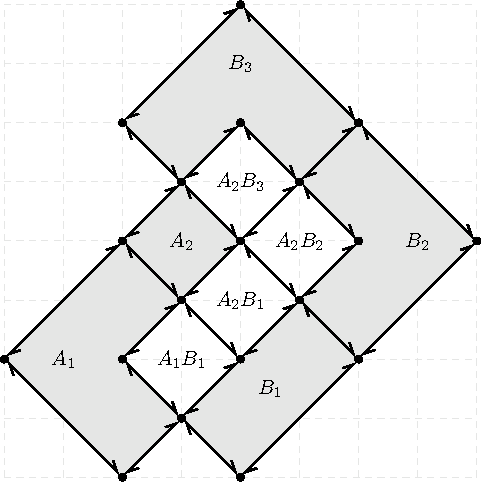
\includegraphics[scale=0.75]{figures/04/DCELDiff}};
    \end{tikzpicture}
}